% --- Classic benchmarks ---
\begin{frame}{MMLU: Massive Multitask Language Understanding}
  \begin{itemize}\footnotesize\itemsep0.3em
    \item[\textcolor{red}{$\blacktriangleright$}] \textbf{15{,}908} four-way multiple-choice questions across \textbf{57 subjects}, from elementary mathematics to professional law and clinical knowledge, grouped into four broad areas: STEM, humanities, social sciences, and ``other''.
    \item[\textcolor{red}{$\blacktriangleright$}] Splits: a \textbf{5-question-per-subject development set} used as the few-shot prompt, a \textbf{1{,}540}-question validation set for hyperparameters, and a \textbf{14{,}079}-question test set (at least 100 test items per subject).
    \item[\textcolor{red}{$\blacktriangleright$}] Standard protocol is \textbf{5-shot}: the prompt opens with ``The following are multiple choice questions (with answers) about \textit{[subject]}.'', appends the five fixed dev examples, then the question, and ends with ``\texttt{Answer: }''.
    \item[\textcolor{red}{$\blacktriangleright$}] What it measures: \textbf{breadth of memorised world knowledge} probed in a rigid format. What it does not measure: generation quality, instruction following, reasoning that takes more than one step, or anything about how the model behaves in a conversation.
    \item[\textcolor{red}{$\blacktriangleright$}] Two cautions worth carrying into any benchmark you read: the paper's own split sizes sum to \textbf{15{,}904}, not the stated 15{,}908; and the per-category task counts differ between the paper's appendix and the released \texttt{categories.py} (they disagree on where \textit{Anatomy} belongs). Small bookkeeping discrepancies are the norm, not the exception.
  \end{itemize}
  \vspace{0.15em}
  {\scriptsize Hendrycks et al., ``Measuring Massive Multitask Language Understanding,'' ICLR 2021, \href{https://arxiv.org/abs/2009.03300v3}{arXiv:2009.03300v3}.}
\end{frame}

\begin{frame}{How Multiple-Choice Scoring Actually Works}
  \begin{columns}[T,onlytextwidth]
    \column{0.52\textwidth}
      \begin{itemize}\scriptsize\itemsep0.05em
        \item[\textcolor{red}{$\blacktriangleright$}] A benchmark is a dataset \textit{plus} a scoring procedure, and the procedure is rarely stated in the headline number. For multiple choice there are three common ones:
        \item[\textcolor{red}{$\blacktriangleright$}] \textbf{Joint:} present all options in the prompt (``A. \ldots\ B. \ldots'') and read off the probability of the \textbf{letter tokens} \texttt{A}--\texttt{D}; predict the argmax. This is MMLU's original method.
        \item[\textcolor{red}{$\blacktriangleright$}] \textbf{Separate:} score each option's \textit{full text} as a continuation, $\log p_\theta(o_j \mid \text{context})$, and take the highest. Often length-normalised. This is what HellaSwag-style harnesses do.
        \item[\textcolor{red}{$\blacktriangleright$}] \textbf{Separate calibrated:} divide out the option's unconditional likelihood, $\log p_\theta(o_j \mid \text{context}) - \log p_\theta(o_j \mid \text{null})$, to stop common strings from winning on prior alone.
        \item[\textcolor{red}{$\blacktriangleright$}] HELM finds the best method is \textbf{determined by the scenario}, and is fairly consistent across models within a scenario. On HellaSwag all six models tested ordered separate $>$ separate-calibrated $>$ joint.
        \item[\textcolor{red}{$\blacktriangleright$}] \textbf{Therefore:} two papers reporting ``MMLU'' can differ by several points from the harness alone. Report the harness and its version.
      \end{itemize}
    \column{0.46\textwidth}
      \centering
      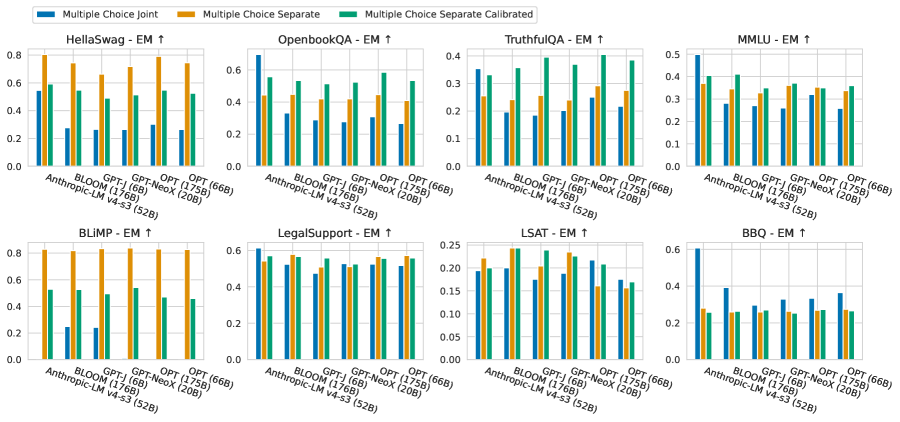
\includegraphics[width=\linewidth,height=0.50\textheight,keepaspectratio]{images/llm-evaluation/helm_fig33_multiple_choice_adaptation.png}\\[0.2em]
      {\scriptsize ``Multiple-choice adaptation. For each adaptation method (joint, separate, and separate calibrated), we compare models across scenarios.'' Liang et al., \href{https://arxiv.org/abs/2211.09110v2}{arXiv:2211.09110v2}, Figure 33.}
  \end{columns}
\end{frame}

\begin{frame}{BIG-Bench and BIG-Bench Hard}
  \begin{itemize}\footnotesize\itemsep0.3em
    \item[\textcolor{red}{$\blacktriangleright$}] \textbf{BIG-Bench} is a community benchmark: \textbf{204 tasks} contributed by \textbf{450 authors} across \textbf{132 institutions}, deliberately chosen to be beyond current capability. \textbf{BIG-Bench Lite} is a 24-task subset for cheaper runs.
    \item[\textcolor{red}{$\blacktriangleright$}] Its lasting methodological contribution is the \textbf{canary string} embedded in every task file --- discussed later under contamination.
    \item[\textcolor{red}{$\blacktriangleright$}] \textbf{BIG-Bench Hard (BBH)} filters BIG-Bench down to \textbf{23 tasks} (27 subtasks, \textbf{6{,}511} examples) through a six-step pipeline; the decisive step keeps only tasks where \textbf{no reported model beat the average human rater}.
    \item[\textcolor{red}{$\blacktriangleright$}] BBH is where \textbf{chain-of-thought prompting} showed its value on a broad suite rather than one dataset:
  \end{itemize}
  \vspace{0.15em}
  \centering
  {\footnotesize
  \begin{tabular}{lccc}
    \toprule
    Model (BBH, 23 tasks) & Answer-only & Chain-of-thought & Tasks above avg.\ human \\
    \midrule
    PaLM 540B                     & 52.3 & \textbf{65.2} & $6 \rightarrow 10$ / 23 \\
    InstructGPT (\texttt{text-davinci-002}) & 51.8 & \textbf{68.4} & $4 \rightarrow 15$ / 23 \\
    Codex (\texttt{code-davinci-002})       & 56.6 & \textbf{73.9} & $5 \rightarrow 17$ / 23 \\
    \bottomrule
  \end{tabular}}

  \vspace{0.25em}
  {\footnotesize \textit{Reference points:} average human rater \textbf{67.7}; max human rater \textbf{94.4}; best prior BIG-Bench result 50.9 (0/23).}

  \vspace{0.3em}
  {\scriptsize Srivastava et al., \href{https://arxiv.org/abs/2206.04615v3}{arXiv:2206.04615v3}; Suzgun et al., ``Challenging BIG-Bench Tasks and Whether Chain-of-Thought Can Solve Them,'' Findings of ACL 2023, \href{https://arxiv.org/abs/2210.09261v1}{arXiv:2210.09261v1}, Table 2.}
\end{frame}

\begin{frame}[allowframebreaks]{HellaSwag and Adversarial Filtering}
  \begin{itemize}\itemsep0.35em
    \item[\textcolor{red}{$\blacktriangleright$}] \textbf{HellaSwag} is commonsense sentence completion: given a context, pick the correct continuation from four. Roughly \textbf{70k} examples in the paper, drawn from ActivityNet captions and WikiHow.
    \item[\textcolor{red}{$\blacktriangleright$}] Its interesting idea is \textbf{Adversarial Filtering (AF)}: generate many wrong endings with a language model, then \textit{iteratively} discard the ones a discriminator (here BERT-Large) finds easy, repartitioning train/test each round. What survives is hard for machines but obvious to people.
    \item[\textcolor{red}{$\blacktriangleright$}] At release the gap was dramatic: humans \textbf{95.6\%} on the test set versus \textbf{47.3\%} for BERT-Large, against 25\% chance. Modern models are above 95\%, so HellaSwag is now a saturated sanity check rather than a discriminating benchmark.
    \item[\textcolor{red}{$\blacktriangleright$}] Two lessons generalise: adversarial filtering is a \textbf{reusable recipe} for making a benchmark harder, and it also \textbf{bakes in the biases of whichever discriminator you filtered against}.
    \item[\textcolor{red}{$\blacktriangleright$}] Bookkeeping caution again: the released dataset has \textbf{59{,}950} rows (train 39{,}905 / validation 10{,}042 / test 10{,}003 with labels withheld), not the 70k quoted in the paper.
  \end{itemize}
  \vspace{0.15em}
  {\scriptsize Zellers et al., ``HellaSwag: Can a Machine Really Finish Your Sentence?'', ACL 2019, \href{https://arxiv.org/abs/1905.07830v1}{arXiv:1905.07830v1}.}
\end{frame}

\begin{frame}{GSM8K: Grade-School Math and Exact-Match Scoring}
  \begin{itemize}\itemsep0.35em
    \item[\textcolor{red}{$\blacktriangleright$}] \textbf{8.5K} linguistically diverse grade-school word problems, split \textbf{7.5K train / 1K test} (the released files actually contain \textbf{7{,}473} and \textbf{1{,}319}). Each takes \textbf{2 to 8 steps} of elementary arithmetic; a bright middle-school student should solve every one.
    \item[\textcolor{red}{$\blacktriangleright$}] Solutions are written in natural language with calculator annotations, and the final number follows a \texttt{\#\#\#\#} delimiter --- documented in the repository rather than the paper:
      \begin{itemize}\footnotesize
        \item[] \texttt{She makes 9 * 2 = \textless{}\textless{}9*2=18\textgreater{}\textgreater{}18 every day at the market.}
        \item[] \texttt{\#\#\#\# 18}
      \end{itemize}
    \item[\textcolor{red}{$\blacktriangleright$}] Scoring is \textbf{generative exact match}: sample a completion, parse out the final number, compare to the key. This is strictly harder than multiple choice --- there is no option list to rank --- and it is why GSM8K became the standard testbed for chain-of-thought.
    \item[\textcolor{red}{$\blacktriangleright$}] It is also where parsing bugs hide. A model that reasons correctly but formats the answer differently scores zero. Always inspect a sample of ``wrong'' generations before believing an exact-match number.
  \end{itemize}
  \vspace{0.15em}
  {\scriptsize Cobbe et al., ``Training Verifiers to Solve Math Word Problems,'' \href{https://arxiv.org/abs/2110.14168v2}{arXiv:2110.14168v2}.}
\end{frame}

\begin{frame}{HumanEval: Execution-Based Evaluation}
  \begin{columns}[T,onlytextwidth]
    \column{0.5\textwidth}
      \begin{itemize}\footnotesize\itemsep0.35em
        \item[\textcolor{red}{$\blacktriangleright$}] \textbf{164 hand-written} Python problems, each with a function signature, docstring, reference body, and unit tests --- an average of \textbf{7.7 tests per problem}.
        \item[\textcolor{red}{$\blacktriangleright$}] The grader is \textbf{the interpreter}, not a string comparison: a sample counts as correct only if it passes every test. This sidesteps the reference-answer problem entirely, which is why execution-based evaluation is the gold standard wherever it is available.
        \item[\textcolor{red}{$\blacktriangleright$}] Hand-writing the problems was deliberate: scraping GitHub would have guaranteed contamination.
        \item[\textcolor{red}{$\blacktriangleright$}] The headline Codex-12B numbers show why sampling budget matters: \textbf{28.8\%} of problems solved with one sample, \textbf{70.2\%} when 100 samples per problem are allowed.
        \item[\textcolor{red}{$\blacktriangleright$}] HumanEval is now saturated and largely superseded by repository-scale suites (SWE-bench) and time-gated ones (LiveCodeBench), but its metric survives everywhere.
      \end{itemize}
    \column{0.48\textwidth}
      \centering
      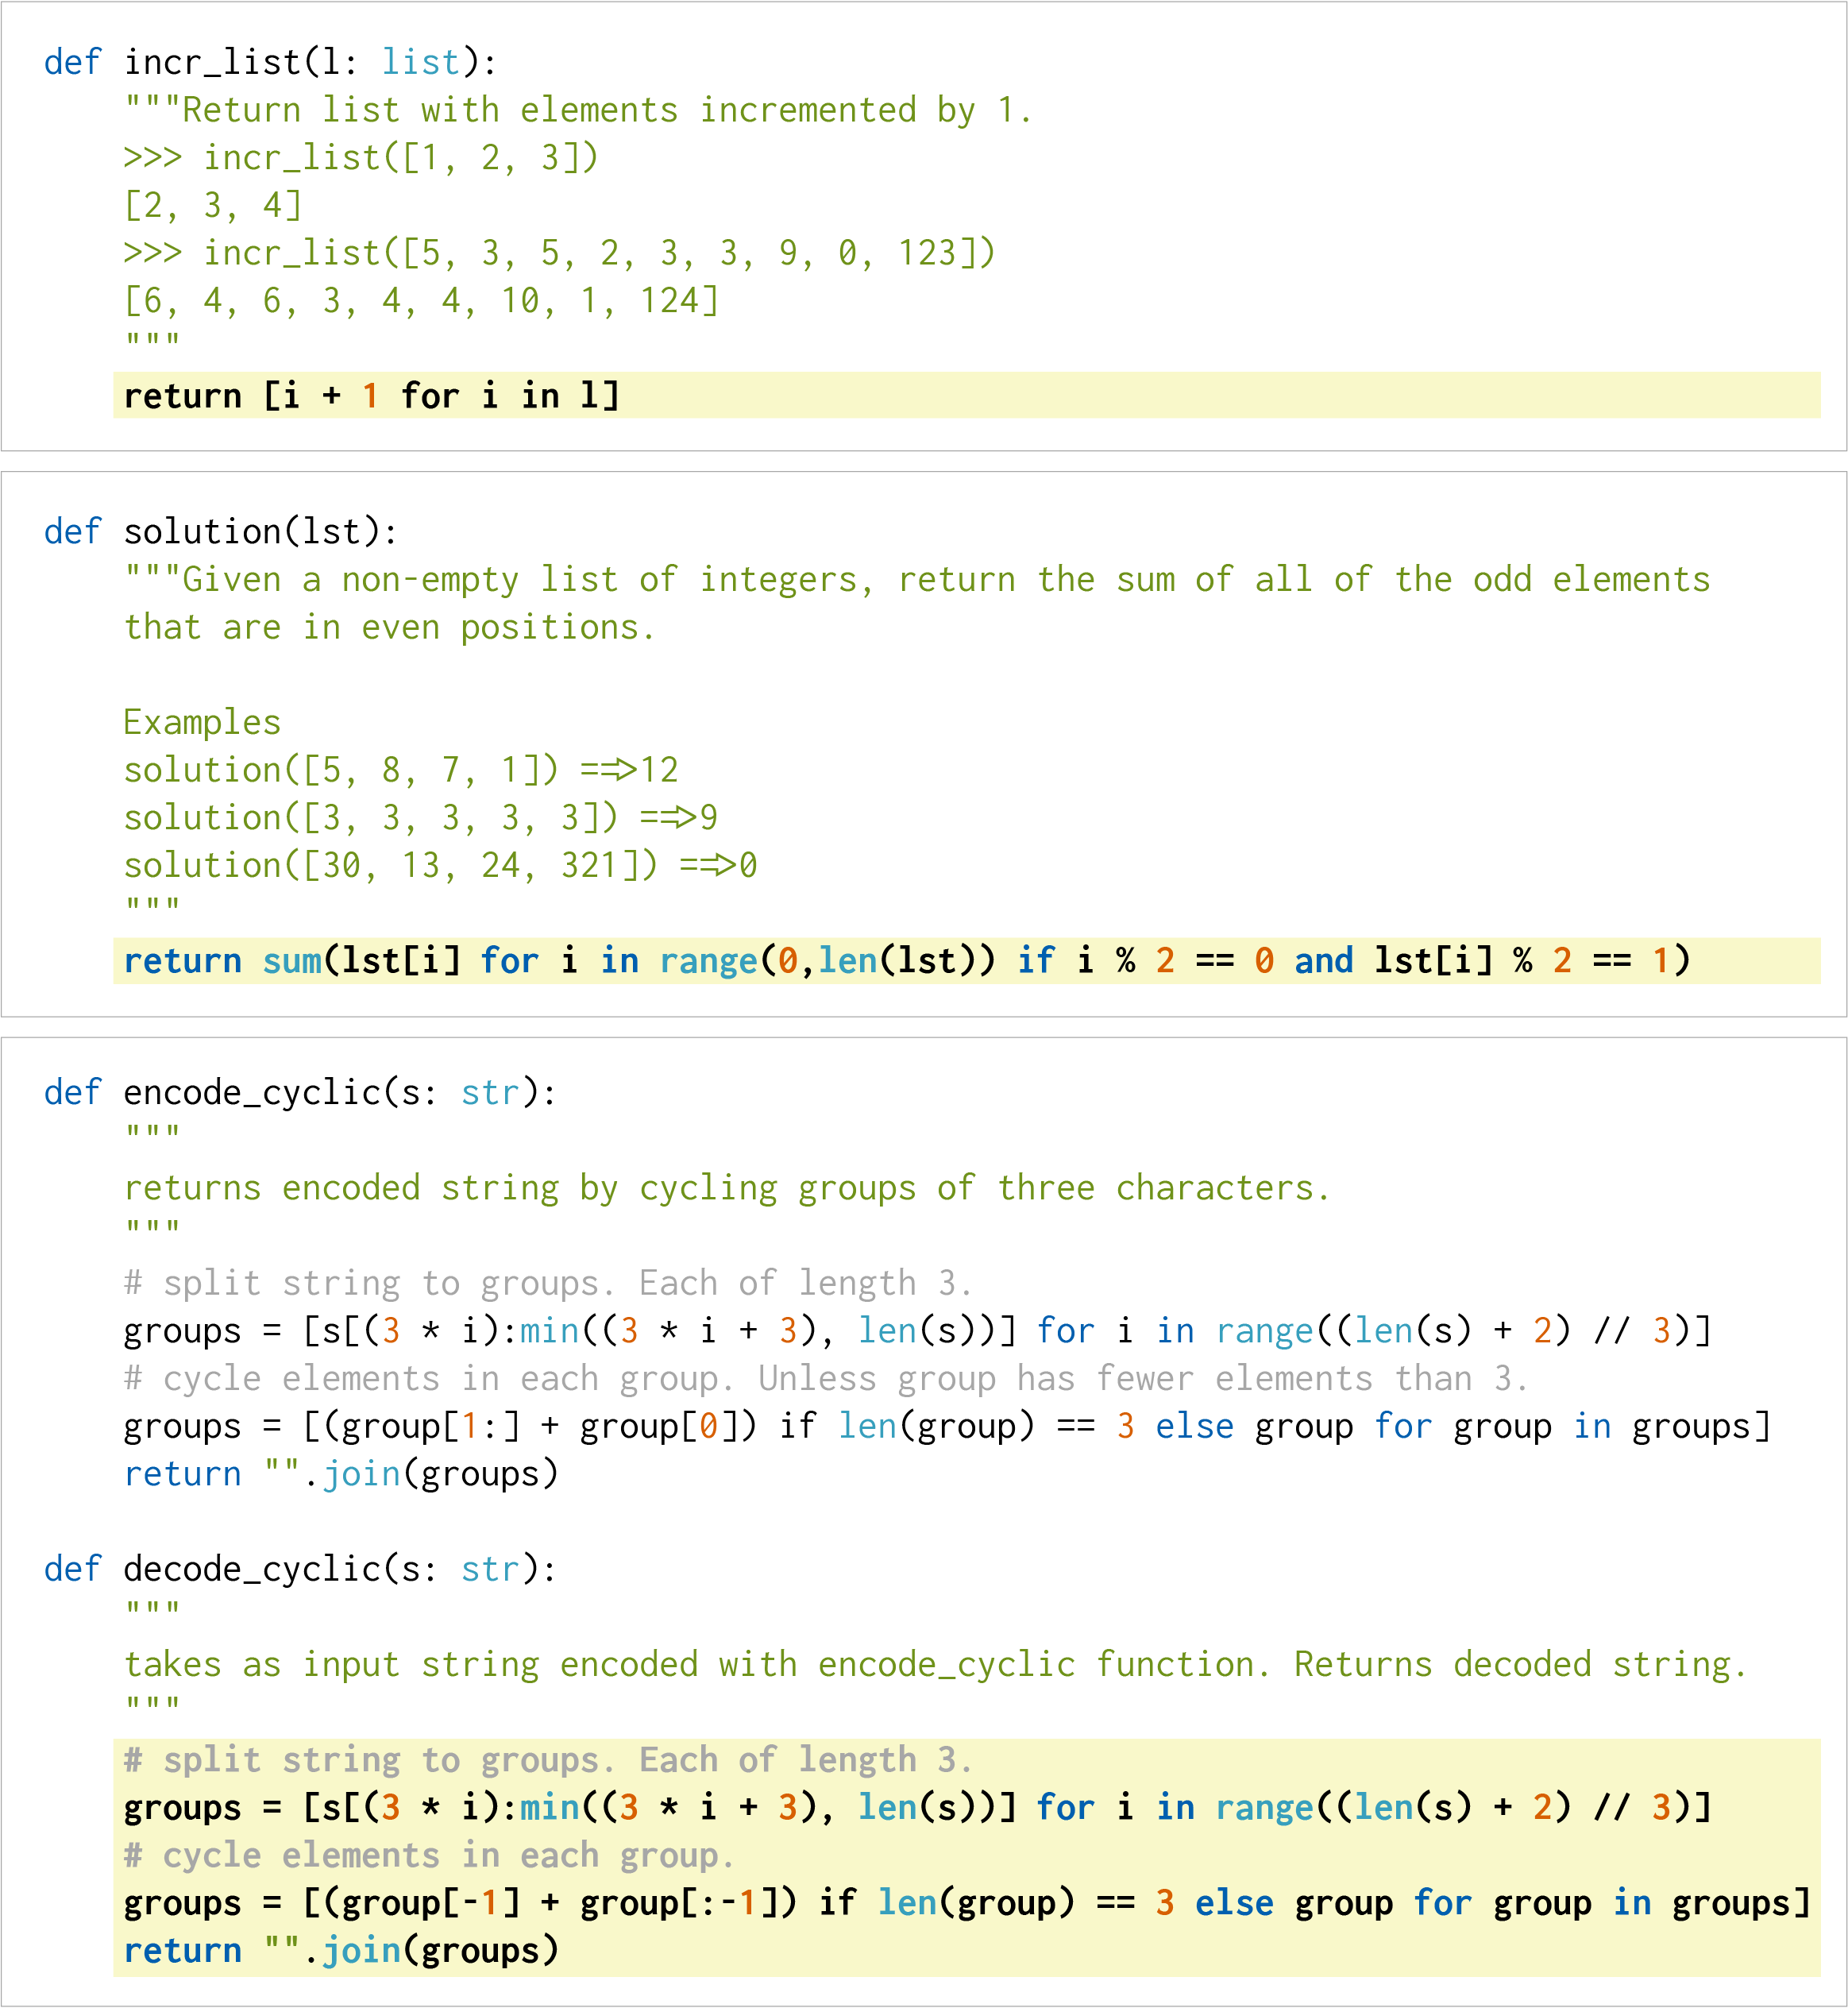
\includegraphics[width=\linewidth,height=0.74\textheight,keepaspectratio]{images/llm-evaluation/humaneval_fig2_example_problems.png}\\[0.1em]
      {\scriptsize ``Three example problems from the HumanEval dataset,'' with the probability that a single Codex-12B sample passes the tests. Chen et al., \href{https://arxiv.org/abs/2107.03374v2}{arXiv:2107.03374v2}, Figure 2.}
  \end{columns}
\end{frame}

\begin{frame}{pass@$k$ and Why the Obvious Estimator Is Wrong}
  \begin{columns}[T,onlytextwidth]
    \column{0.54\textwidth}
      \begin{itemize}\scriptsize\itemsep0.05em
        \item[\textcolor{red}{$\blacktriangleright$}] \textbf{Definition.} Generate $k$ samples per problem; the problem counts as solved if \textit{any} sample passes; pass@$k$ is the fraction of problems solved.
        \item[\textcolor{red}{$\blacktriangleright$}] Computed that way the estimate has high variance, so the paper generates $n \geq k$ samples, counts the $c \leq n$ that pass, and uses the \textbf{unbiased estimator}
          \[
            \text{pass@}k := \mathop{\mathbb{E}}_{\text{problems}}\left[\,1 - \frac{\binom{n-c}{k}}{\binom{n}{k}}\,\right],
          \]
          the probability that a random size-$k$ subset of the $n$ samples is not entirely drawn from the $n-c$ failures. They use $n = 200$, $k \leq 100$.
        \item[\textcolor{red}{$\blacktriangleright$}] The tempting shortcut $1 - (1-\hat{p})^k$ with $\hat{p} = c/n$ is \textbf{biased downwards}, and the bias does not vanish with more samples --- it is a consequence of plugging an estimate into a non-linear function (Jensen's inequality), not of small $n$.
        \item[\textcolor{red}{$\blacktriangleright$}] Compute the binomial ratio in \textbf{log space} or with the cancelling-product form; the factorials overflow immediately at $n=200$.
        \item[\textcolor{red}{$\blacktriangleright$}] pass@$k$ rewards \textbf{coverage under sampling}. Its sibling pass\textasciicircum$k$ (all $k$ samples succeed) measures \textbf{consistency} and is the right choice for agent reliability.
      \end{itemize}
    \column{0.44\textwidth}
      \centering
      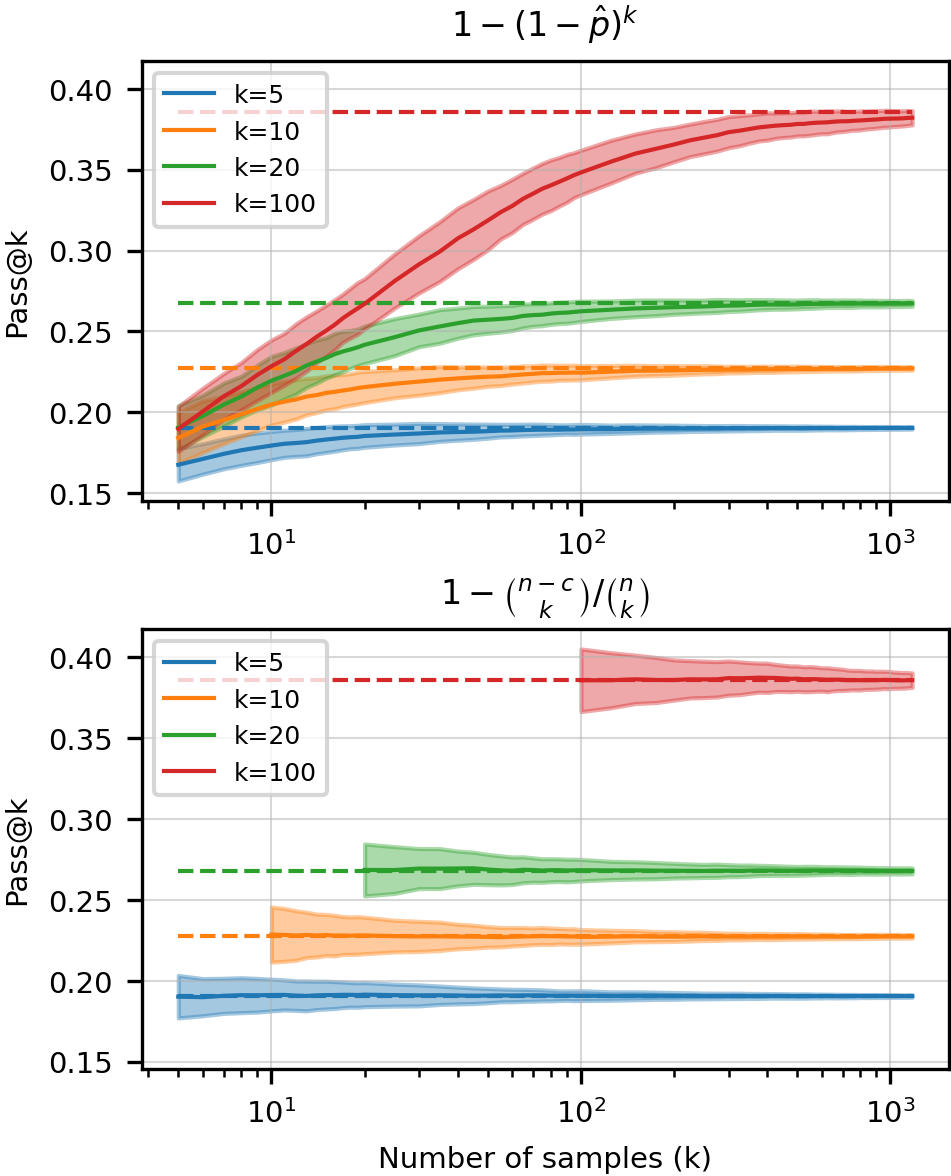
\includegraphics[width=0.92\linewidth,height=0.54\textheight,keepaspectratio]{images/llm-evaluation/humaneval_fig13_passk_estimator.png}\\[0.1em]
      {\scriptsize Bias and variance of the two pass@$k$ estimators: ``the gap doesn't fully close even when $n > 5k$.'' Chen et al., \href{https://arxiv.org/abs/2107.03374v2}{arXiv:2107.03374v2}, Figure 13.}
  \end{columns}
\end{frame}

\begin{frame}{Choosing a Scoring Mode}
  \begin{itemize}\footnotesize
    \item[\textcolor{red}{$\blacktriangleright$}] The scoring mode, not the dataset, decides what a benchmark can tell you and how it can be gamed.
  \end{itemize}
  \vspace{0.3em}
  {\centering\scriptsize
  \begin{tabular}{p{2.25cm} p{3.0cm} p{2.75cm} p{3.35cm}}
    \toprule
    \textbf{Mode} & \textbf{How it scores} & \textbf{Examples} & \textbf{Main failure mode} \\
    \midrule
    Multiple-choice likelihood & Rank options by model probability; no free generation & MMLU, HellaSwag, ARC & Sensitive to option order, format, and calibration; unlike real usage \\
    \addlinespace[0.2em]
    Generative exact match & Sample, parse, compare to a key & GSM8K, TriviaQA, IFEval & Parsing bugs; punishes correct answers in the wrong format \\
    \addlinespace[0.2em]
    Execution / verification & Run code or a checker against tests & HumanEval, SWE-bench, LiveCodeBench & Test suites can be incomplete; only applies to checkable domains \\
    \addlinespace[0.2em]
    Model-graded (judge) & A strong LLM scores or ranks outputs & MT-Bench, AlpacaEval, RAGAS & Judge biases (position, verbosity, self-preference); needs calibration \\
    \addlinespace[0.2em]
    Human preference & People vote or grade against a rubric & Chatbot Arena, expert review & Expensive, slow, noisy; agreement must be measured \\
    \bottomrule
  \end{tabular}\par}
  \vspace{0.5em}
  \begin{itemize}\footnotesize
    \item[\textcolor{red}{$\blacktriangleright$}] Rule of thumb: use the \textbf{cheapest mode that can actually fail} for your task. Reach for a judge only when no verifier exists, and for humans only when the judge itself is in question.
  \end{itemize}
\end{frame}
